\documentclass{beamer}
\usepackage[utf8]{inputenc}

\usetheme{Madrid}
\usecolortheme{default}
\usepackage{amsmath,amssymb,amsfonts,amsthm}
\usepackage{txfonts}
\usepackage{tkz-euclide}
\usepackage{listings}
\usepackage{adjustbox}
\usepackage{array}
\usepackage{tabularx}
\usepackage{gvv}
\usepackage{lmodern}
\usepackage{circuitikz}
\usepackage{tikz}
\usepackage{graphicx}
\usepackage{multicol}

\setbeamertemplate{page number in head/foot}[totalframenumber]

\usepackage{tcolorbox}
\tcbuselibrary{minted,breakable,xparse,skins}

\definecolor{bg}{gray}{0.95}
\DeclareTCBListing{mintedbox}{O{}m!O{}}{%
  breakable=true,
  listing engine=minted,
  listing only,
  minted language=#2,
  minted style=default,
  minted options={%
    linenos,
    gobble=0,
    breaklines=true,
    breakafter=,,
    fontsize=\small,
    numbersep=8pt,
    #1},
  boxsep=0pt,
  left skip=0pt,
  right skip=0pt,
  left=25pt,
  right=0pt,
  top=3pt,
  bottom=3pt,
  arc=5pt,
  leftrule=0pt,
  rightrule=0pt,
  bottomrule=2pt,
  toprule=2pt,
  colback=bg,
  colframe=orange!70,
  enhanced,
  overlay={%
    \begin{tcbclipinterior}
    \fill[orange!20!white] (frame.south west) rectangle ([xshift=20pt]frame.north west);
    \end{tcbclipinterior}},
  #3,
}
\lstset{
    language=C,
    basicstyle=\ttfamily\small,
    keywordstyle=\color{blue},
    stringstyle=\color{orange},
    commentstyle=\color{green!60!black},
    numbers=left,
    numberstyle=\tiny\color{gray},
    breaklines=true,
    showstringspaces=false,
}

\numberwithin{equation}{section}
\lstset{
  language=Python,
  basicstyle=\ttfamily\small,
  keywordstyle=\color{blue},
  stringstyle=\color{orange},
  numbers=left,
  numberstyle=\tiny\color{gray},
  breaklines=true,
  showstringspaces=false
}



\title{Problem 4.4.26}
\author{Sarvesh Tamgade}

\date{\today} 
\begin{document}

\begin{frame}
\titlepage
\end{frame}

\section{Question}
\begin{frame}{Question}
 Find the equation of the median through vertex \(\vec{A}\) of the triangle \(ABC\), having vertices
\[
\vec{A}(2,5), \quad \vec{B}(-4,9), \quad \vec{C}(-2,-1).
\]

\end{frame}

\section{Solution}
\begin{frame}[fragile]
    \frametitle{Solution}
\textbf{Solution:} \\

Using the section formula, the midpoint \(\vec{M}\) of the side \(BC\) is
\[
\vec{M} = \frac{\vec{B} + \vec{C}}{2} = 
\frac{1}{2} \myvec{-4 \\ 9} + 
\frac{1}{2} \myvec{-2 \\ -1} = 
\myvec{-3 \\ 4}.
\tag{0.1}
\]

The median passes through points \(\vec{A} = \myvec{2 \\ 5}\) and \(\vec{M} = \myvec{-3 \\ 4}\).

Let the required line have the equation
\[
\vec{n}^\top \vec{x} = 1,
\tag{0.2}
\]
where
\[
\vec{n} = \myvec{n_1 \\ n_2}
\tag{0.3}
\]
is the column vector (normal vector).


\end{frame}
\begin{frame}[fragile]
    \frametitle{Solution}

Since both points \(\vec{A}\) and \(\vec{M}\) lie on the median, they satisfy the line equation:
\[
\vec{n}^\top \vec{A} = 1, \quad \vec{n}^\top \vec{M} = 1,
\tag{0.4}
\]
or, explicitly,
\[
\myvec{2 & 5 \\ -3 & 4} \vec{n} = \myvec{1 \\ 1}.
\tag{0.5}
\]

We want to find \(\vec{n}\) satisfying
\[
\myvec{2 & 5 \\ -3 & 4} \vec{n} = \vec{c},
\quad \text{where } \vec{c} = \myvec{1 \\ 1}.
\tag{0.6}
\]

Set up the augmented matrix with right-hand side \(1\):
\[
\myaugvec{2}{
2 & 5 & 1 \\
-3 & 4 & 1
}
\tag{0.7}
\]

Perform row operation \(R_2 \to R_2 + \frac{3}{2} R_1\):

\end{frame}
\begin{frame}[fragile]
    \frametitle{Solution}
\[
\myaugvec{2}{
2 & 5 & 1 \\
0 & \frac{23}{2} & \frac{5}{2}
}
\tag{0.8}
\]

Perform row operation \(R_1 \to R_1 - \frac{10}{23} R_2\):
\[
\myaugvec{2}{
2 & 0 & -\frac{2}{23} \\
0 & \frac{23}{2} & \frac{5}{2}
}
\tag{0.9}
\]

The final augmented matrix is:
\[
\myaugvec{2}{
2 & 0 & -\frac{2}{23} \\
0 & \frac{23}{2} & \frac{5}{2}
}
\tag{0.10}
\]

Solve the system:
\[
2 n_1 = -\frac{2}{23} \implies n_1 = -\frac{1}{23}
\tag{0.11}
\]

\[
\frac{23}{2} n_2 = \frac{5}{2} \implies n_2 = \frac{5}{23}
\tag{0.12}
\]

\end{frame}
\begin{frame}[fragile]
    \frametitle{Solution}

\[
\vec{n} = \frac{1}{23} \myvec{-1 \\ 5}
\tag{0.13}
\]

Therefore, equation of required line is:
\[
\boxed{
\myvec{-1 & 5} \vec{x} = 23
}
\]


\end{frame}
\section{Graph}
\begin{frame}
    \frametitle{Graph}
    \begin{figure}[htbp]
    \centering
    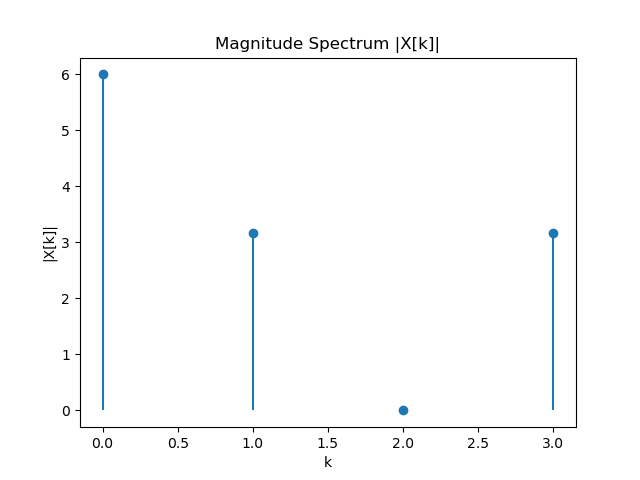
\includegraphics[width=0.65\linewidth]{FIG/fig1.png}
    \caption{Vector Representation}
    \label{fig:FIG/fig1.png}
\end{figure}
\end{frame}
\section{ C Code}
\begin{frame}[fragile]
\frametitle{C Code }
\begin{lstlisting}[language=C]
#include <stdio.h>
#include "trianglefun.h"

int main() {
    // Vertices of triangle
    int Ax = 2, Ay = 5;
    int Bx = -4, By = 9;
    int Cx = -2, Cy = -1;

    char equation[50];

    // Calculate the median equation and store as string
    median_equation(Ax, Ay, Bx, By, Cx, Cy, equation);

    // Print the equation
    printf("Equation of the median from A: %s\n", equation);

    return 0;
}



    
\end{lstlisting}
\end{frame}


\begin{frame}[fragile]
\frametitle{Python Code for Plotting}
\begin{lstlisting}[language=Python]
import matplotlib.pyplot as plt
import numpy as np

# Vertices of the triangle
A = np.array([2, 5])
B = np.array([-4, 9])
C = np.array([-2, -1])

# Calculate midpoint M of BC
M = (B + C) / 2

# Plot triangle
plt.figure(figsize=(6,6))
triangle_points = np.array([A, B, C, A])
plt.plot(triangle_points[:,0], triangle_points[:,1], 'k-', label='Triangle ABC')

# Plot vertices
plt.plot(A[0], A[1], 'ro')

\end{lstlisting}

\end{frame}
\begin{frame}[fragile]
\frametitle{Python Code for Plotting}
\begin{lstlisting}[language=Python]
plt.plot(B[0], B[1], 'ro')
plt.plot(C[0], C[1], 'ro')

# Label vertices
plt.text(A[0]+0.2, A[1], 'A(2,5)', fontsize=12, color='red')
plt.text(B[0]+0.2, B[1], 'B(-4,9)', fontsize=12, color='red')
plt.text(C[0]+0.2, C[1], 'C(-2,-1)', fontsize=12, color='red')

# Plot median from A to midpoint M
plt.plot([A[0], M[0]], [A[1], M[1]], 'b--', linewidth=2, label='Median AM')

# Label midpoint M
plt.plot(M[0], M[1], 'go')
plt.text(M[0]+0.2, M[1], f'M({M[0]:.1f},{M[1]:.1f})', fontsize=12, color='green')

# Position to place equation on the median line midpoint
mid_x = (A[0] + M[0]) / 2

\end{lstlisting}

\end{frame}
\begin{frame}[fragile]
\frametitle{Python Code for Plotting}
\begin{lstlisting}[language=Python]

mid_y = (A[1] + M[1]) / 2

# Settings
plt.gca().set_aspect('equal', adjustable='box')
plt.grid(True)
plt.legend()
plt.title('Triangle ABC with Median from A')
plt.xlabel('X-axis')
plt.ylabel('Y-axis')
plt.xlim(-6, 4)
plt.ylim(-3, 11)

# Save the figure as PNG
filename = 'triangle_median_eqonline.png'
plt.savefig(filename)
plt.close()
\end{lstlisting}

\end{frame}
\begin{frame}[fragile]
    \frametitle{Python Code - Using Shared Object}
    \begin{lstlisting}
import numpy as np
import matplotlib.pyplot as plt
import ctypes

# Load the shared object for triangle median equation
triangle_lib = ctypes.CDLL("./trianglefun.so")

# Define the function prototype for median_equation
triangle_lib.median_equation.argtypes = [ctypes.c_int, ctypes.c_int, ctypes.c_int, ctypes.c_int, ctypes.c_int, ctypes.c_int, ctypes.c_char_p]

# Triangle vertices (same as in C main program)
Ax, Ay = 2, 5
Bx, By = -4, 9
Cx, Cy = -2, -1


\end{lstlisting}
\end{frame}

\begin{frame}[fragile]
    \frametitle{Python Code - Using Shared Object}
    \begin{lstlisting}
# Prepare a ctypes buffer to store the median equation string
buffer = ctypes.create_string_buffer(50)

# Call C function
triangle_lib.median_equation(Ax, Ay, Bx, By, Cx, Cy, buffer)

# Get median equation string from buffer
median_eqn = buffer.value.decode('utf-8')

# Calculate midpoint M of BC (for plotting)
M = np.array([(Bx + Cx) / 2, (By + Cy) / 2])
A = np.array([Ax, Ay])

# Plot triangle
plt.figure(figsize=(6,6))
triangle_points = np.array([A, [Bx, By], [Cx, Cy], A])
plt.plot(triangle_points[:,0], triangle_points[:,1], 'k-', label='Triangle ABC')


\end{lstlisting}
\end{frame}
\begin{frame}[fragile]
    \frametitle{Python Code - Using Shared Object}
    \begin{lstlisting}
# Plot vertices
plt.plot(Ax, Ay, 'ro')
plt.plot(Bx, By, 'ro')
plt.plot(Cx, Cy, 'ro')

# Label vertices
plt.text(Ax+0.2, Ay, f'A({Ax},{Ay})', fontsize=12, color='red')
plt.text(Bx+0.2, By, f'B({Bx},{By})', fontsize=12, color='red')
plt.text(Cx+0.2, Cy, f'C({Cx},{Cy})', fontsize=12, color='red')

# Plot median from A to midpoint M
plt.plot([Ax, M[0]], [Ay, M[1]], 'b--', linewidth=2, label='Median AM')

# Label midpoint M
plt.plot(M[0], M[1], 'go')
plt.text(M[0]+0.2, M[1], f'M({M[0]:.1f},{M[1]:.1f})', fontsize=12, color='green')


\end{lstlisting}
\end{frame}

\begin{frame}[fragile]
    \frametitle{Python Code - Using Shared Object}
    \begin{lstlisting}

# Position to place equation near the median line midpoint
mid_x = (Ax + M[0]) / 2
mid_y = (Ay + M[1]) / 2

# Show median equation at midpoint
plt.text(mid_x, mid_y, median_eqn, fontsize=14, color='blue')

# Settings
plt.gca().set_aspect('equal', adjustable='box')
plt.grid(True)
plt.legend()


\end{lstlisting}
\end{frame}
\begin{frame}[fragile]
    \frametitle{Python Code - Using Shared Object}
    \begin{lstlisting}


plt.title('Triangle ABC with Median from A')
plt.xlabel('X-axis')
plt.ylabel('Y-axis')
plt.xlim(-6, 4)
plt.ylim(-3, 11)

# Save and show plot
plt.savefig('triangle_median_eqonline_from_c.png')
plt.show()


\end{lstlisting}
\end{frame}


\begin{frame}{Plot-Using Both C and Python}
    \centering
    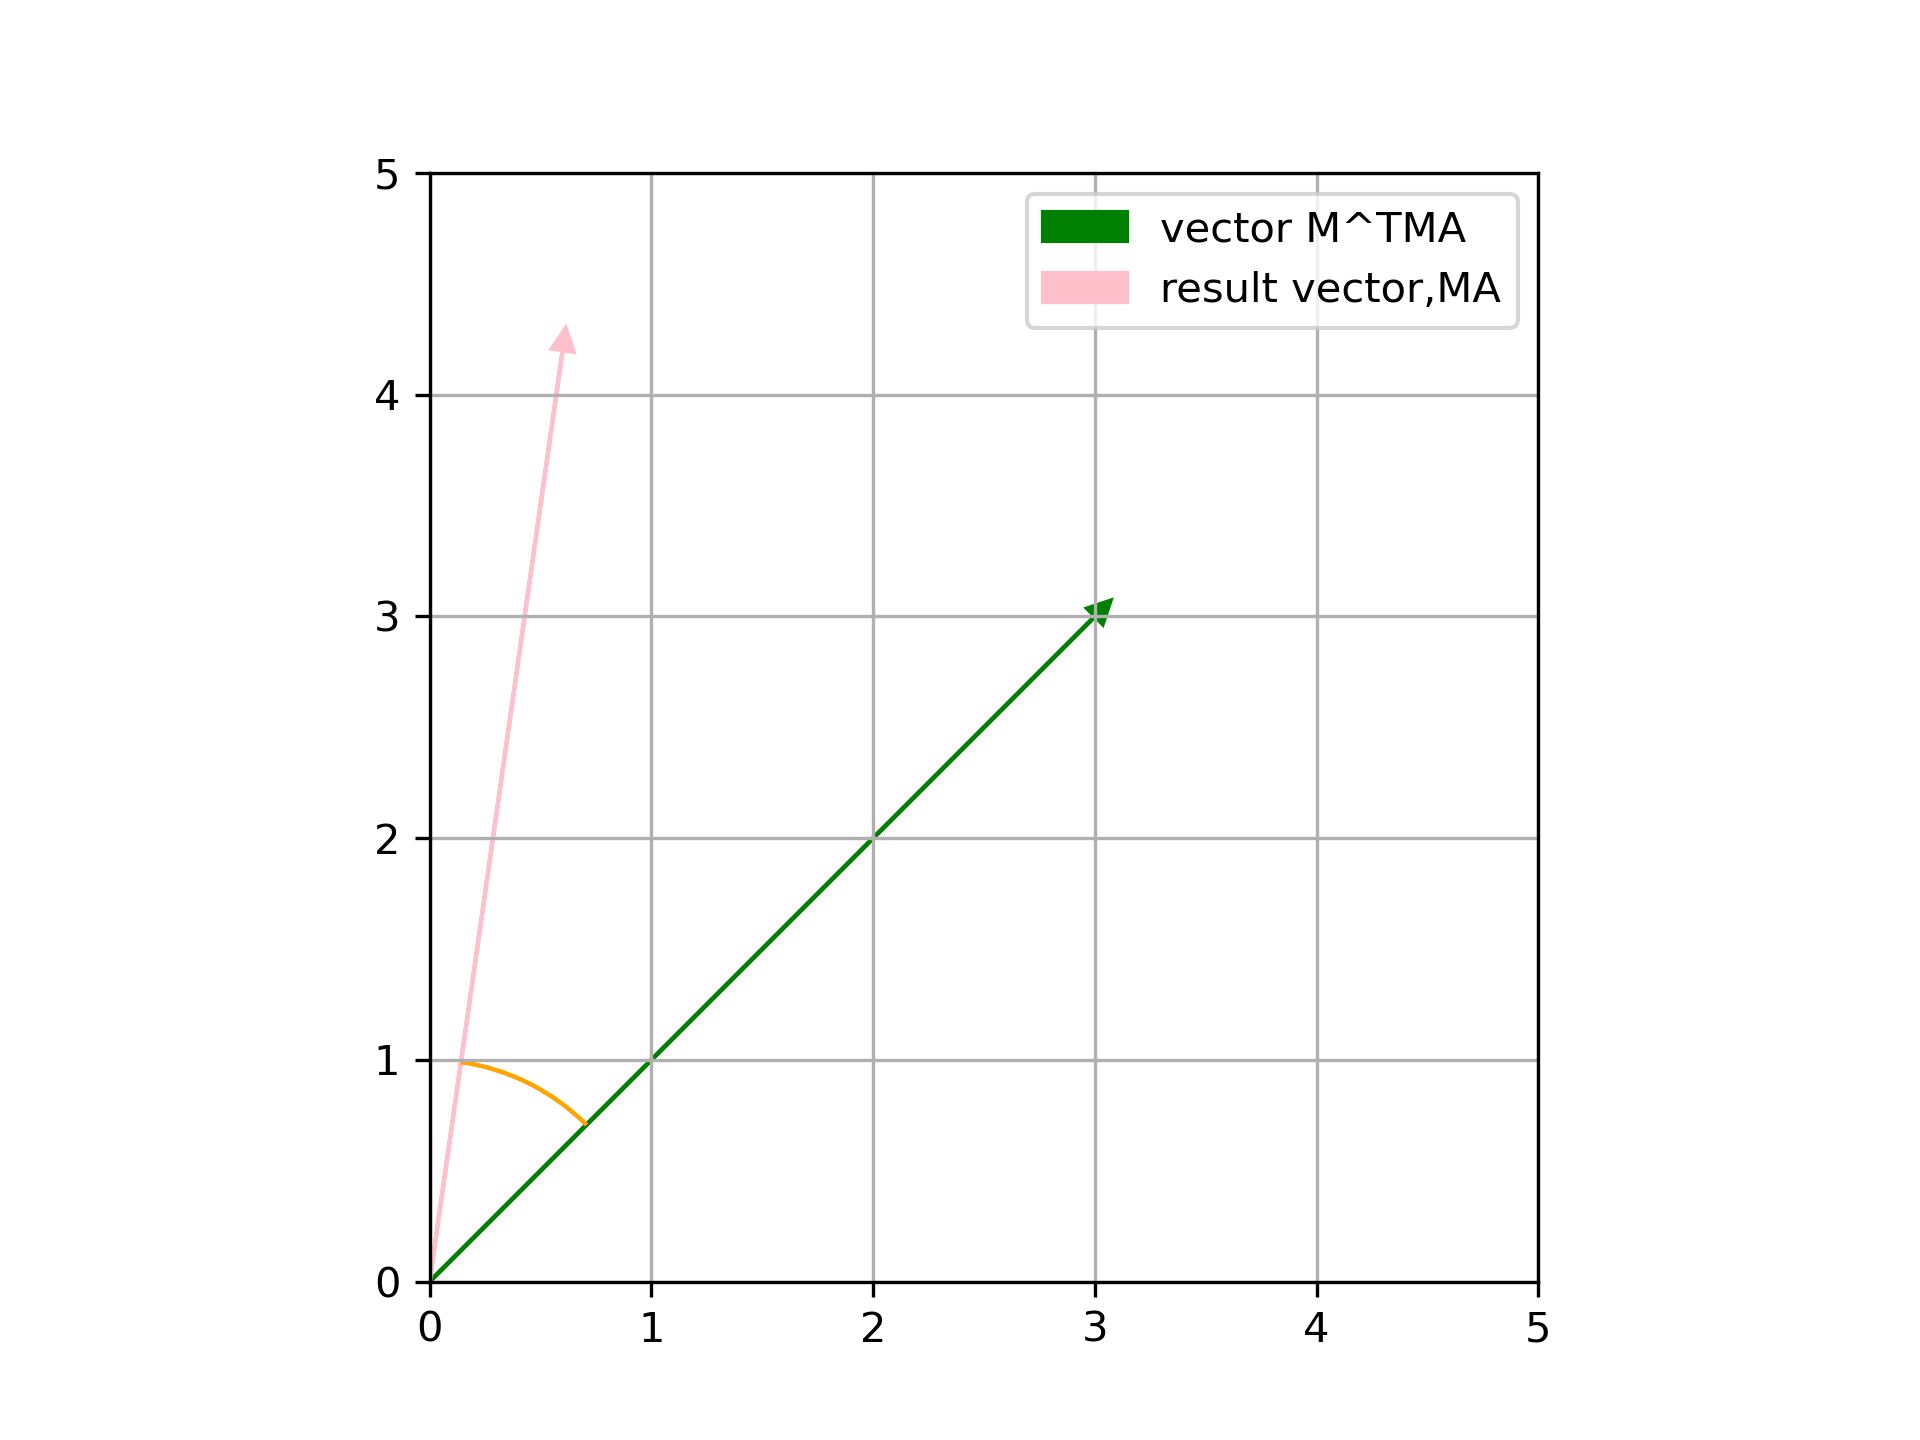
\includegraphics[width=\columnwidth, height=0.8\textheight, keepaspectratio]{FIG/fig2.png}     
\end{frame}


\end{document}
